\documentclass[book.tex]{subfiles}
\begin{document}
id Software was funded during February 1991 by four people: 

 \begin{figure}[H]
\centering  
\begin{tabularx}{\textwidth}{ X  X  X  }
  \toprule
  \textbf{Name} &  \textbf{Age} & \textbf{Occupation} \\
  \toprule 
   John Carmack & 22 &  Programming\\
   John Romero & 25 &  Programming\\
   Adrian Carmack & 22 &  Artist\\
   Tom Hall & 28 &  Creative Director\\
     \toprule
\end{tabularx}
\caption{id Software founding members.}\label{fig:Id Software team}
\end{figure}

Wolfenstein 3D was id first title but the team had already shipped no less than 13 games will working for their previous employer SoftDisk:\\
\begin{itemize}
  \item Dangerous Dave (1988)\footnote{Dangerous Dave is a solo project of John Romero predating Id's formation, but Id Software produced its first sequel and it is sometimes regarded as an early Id Software title. Later Dangerous Dave sequels were not made by Id, nor were later Catacomb titles.}
  \item Commander Keen
  \begin{itemize}
    \item Episode 1: Marooned on Mars (1990)
    \item Episode 2: The Earth Explodes (1991)
    \item Episode 3: Keen Must Die (1991)
    \item Keen Dreams (1991)
    \item Episode 4: Secret of the Oracle (1991)
    \item Episode 5: The Armageddon Machine (1991)
    \item Episode 6: Aliens Ate My Baby Sitter (1991)
  \end{itemize}
  
  \item Dangerous Dave in the Haunted Mansion (1991)
  \item Rescue Rover (1991)
  \item Rescue Rover 2 (1991)
  \item Shadow Knights (1991)
  \item Hovertank 3D (1991)
  \item Catacomb 3D: A New Dimension (1991)
\end{itemize}


Considering the magnitude and ambitions of the title, four more people were added to the team for a total of eight.\\

 \begin{figure}[H]
\centering  
\begin{tabularx}{\textwidth}{ X  X  X  }
  \toprule
  \textbf{Name} &  \textbf{Age} & \textbf{Occupation} \\
  \toprule 
   Jay Wilbur & ?? &  Business\\
   Kevin Cloud & 27 &  Computer Artist\\
   Robert Prince & ?? &  Composer\\
   Jason Blochowiak & ?? &   Programming\\
     \toprule
\end{tabularx}
\caption{id Software new hires.}\label{fig:Id Software hires}
\end{figure}

\begin{fancyquotes}
Jason was part of Id at the start, but we parted ways during Wolf development\footnote{Jason still wrote part of the memory manager and is credited for introducing John Carmack to Unix development which ultimately led to the purchase of a Next Color ColorStation}.
 \bigskip \\
\textbf{John Carmack - Programmer}
 \end{fancyquotes}
 
\begin{figure}[H]
\centering
  \shadowbox{
      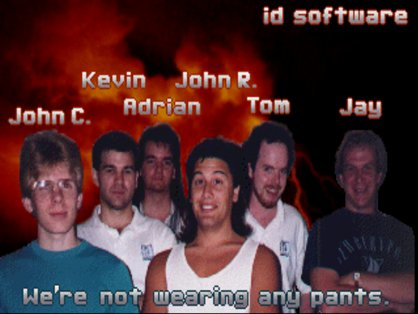
\includegraphics[width=\textwidth]{imgs/idTeam_team_pants.png}
  }  
\caption{id software team circa 1993 as show from Wolfenstein 3D.}
\label{fig:id_team_1993}
\end{figure}
 
\begin{figure}[H]
\centering
  \shadowbox{
      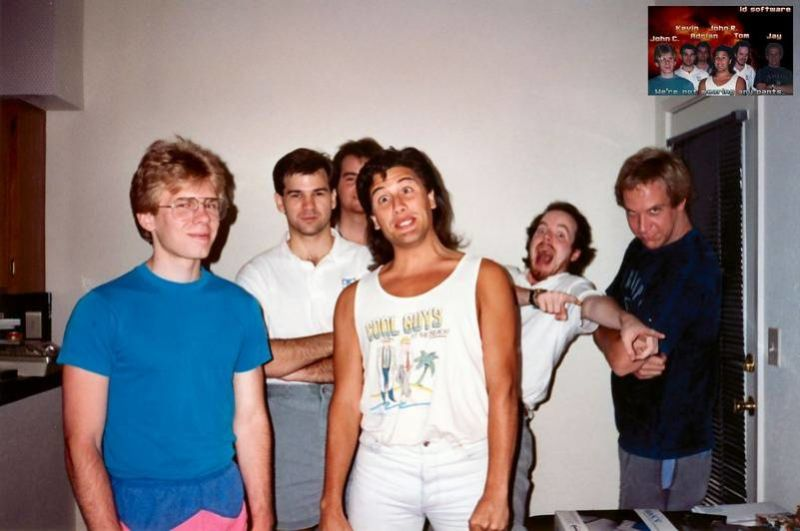
\includegraphics[width=\textwidth]{imgs/id_team_with_pants.jpg}
  }  
\caption{They were in fact wearing pants.}
\label{fig:id_team_1993}
\end{figure}

Every member was working with an high end 386-DX 33Mhz. As for combining engine, tools and assets:\\

 \begin{fancyquotes}
We started with floppy data transfer, but we had a Novell network on coax Ethernet by the end. We didn't have a version control system.  Surprisingly, we went all the way to Quake 3 without one, then we started using Visual Source Safe.\\
 \\
\textbf{John Carmack - Programmer}
\end{fancyquotes}







During Wold3D development (from November 1991 to May 1992: Roughly six months), id Software was located in Madison, WI
\begin{figure}[H]
\centering
 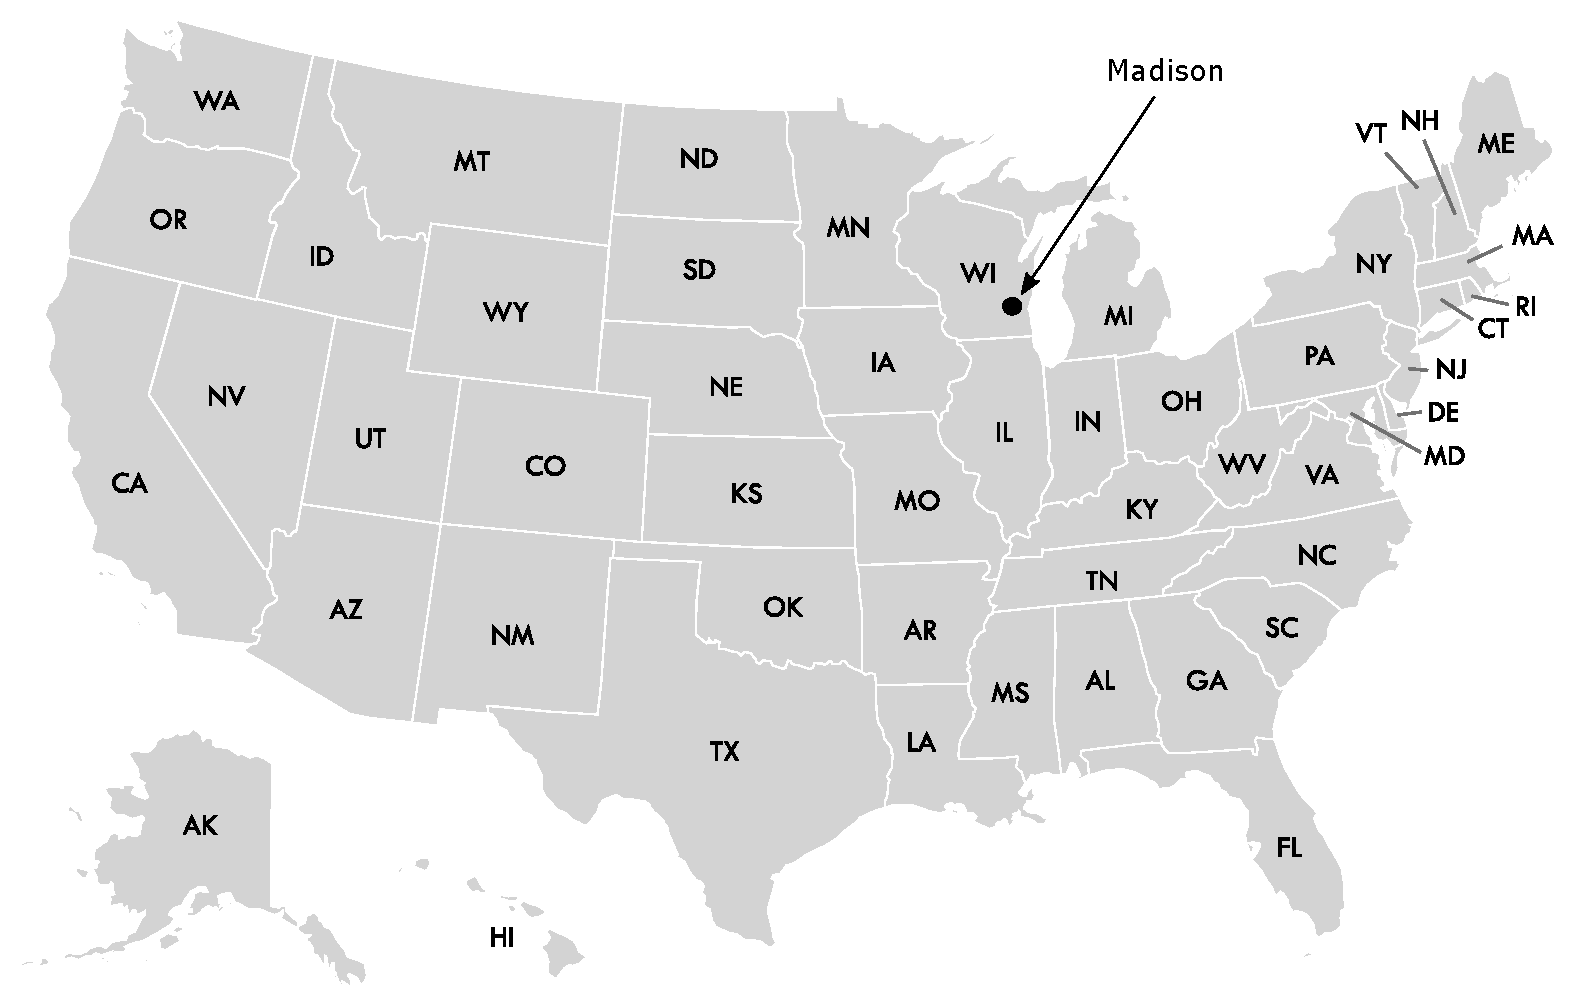
\includegraphics[width=\textwidth]{map/usa-id-software.eps}
 \end{figure}









\section{Programming}



Development was done with Borland C++ 3.1 (the language used however was C): The editor used VGA mode 3: 80 characters wide and 25 characters tall.

John Carmack took care of the runtime code. John Romero programmed many of the tools (editor, packers, ...). Jason Blochowiak was contracted to write important subsystems of the game (Input manager, Page Manager, Sound Manager, User Manager).\\
\\
\begin{figure}[H]
\centering
  \shadowbox{
      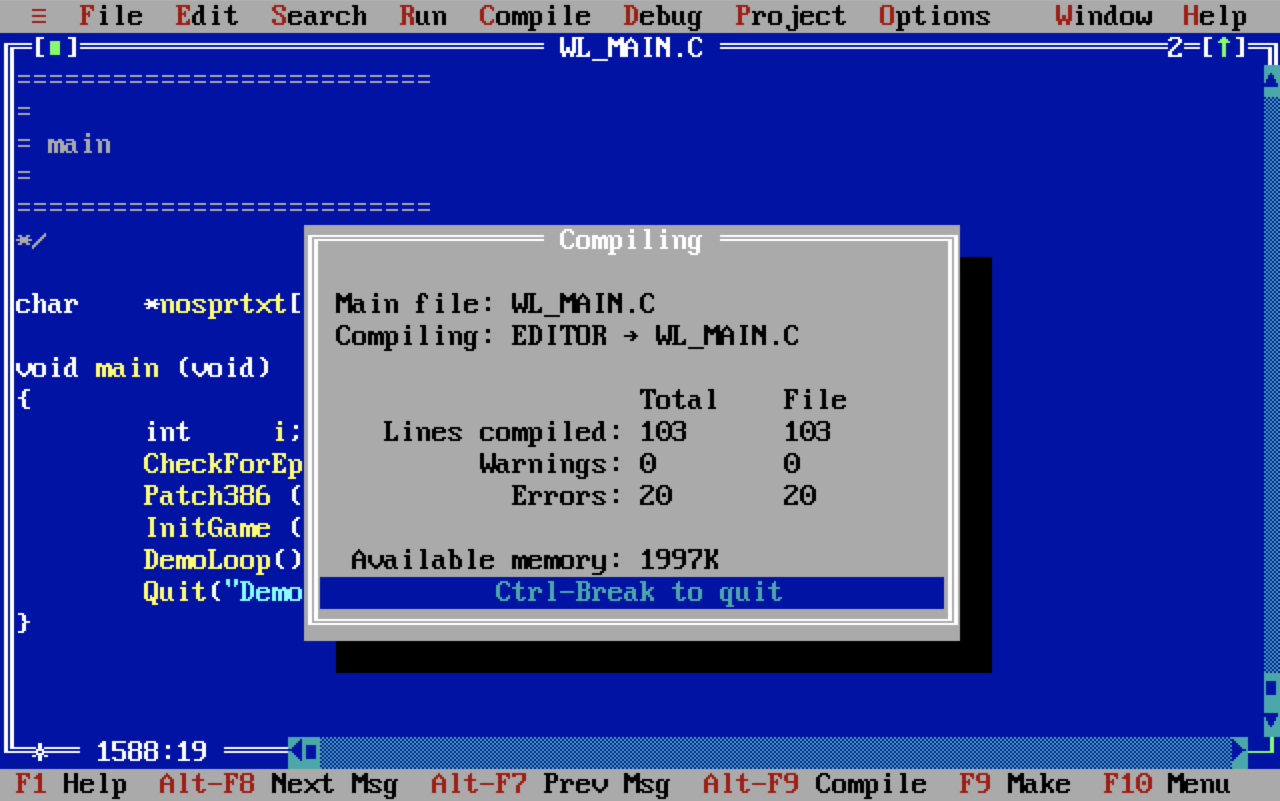
\includegraphics[width=\textwidth]{screenshots/development.png}
  }  
\caption{Bordland C++ 3.1 editor}
\end{figure}


To compensate for the tiny CRT, some of the developers used two screens (an unusual thing at the time).\\

\begin{fancyquotes}
At that point, we wanted 21" monitors, but couldn't justify them.  I used a second mono monitor to allow Turbo Debugger 386 to keep the main screen in graphics mode while I stepped through the code.\\
 \\
\textbf{John Carmack - Programmer}
\end{fancyquotes}
\\
You may have noticed in the listing of VGA mode 13h and 4h (See figure~\ref{fig:vga_modes} on page~\pageref{fig:vga_modes}): they don't have the same starting segment. This allows to plug two graphi cards in the PC: One in monochrome text and the other one in regular VGA. This allows a developer to debug the game engine in real-time.\\
\begin{figure}[H]
\centering
  \shadowbox{
      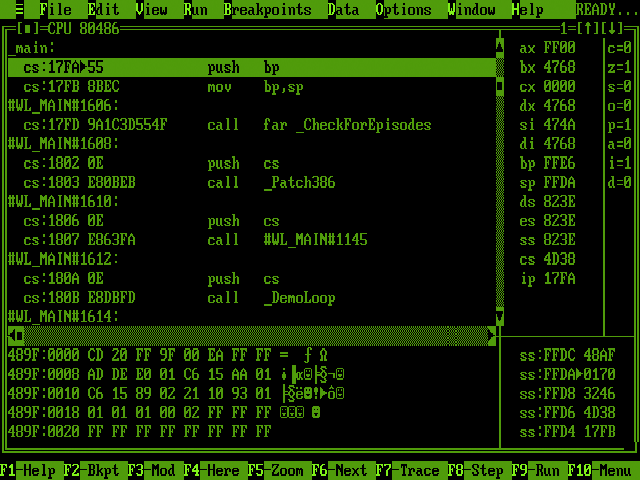
\includegraphics[width=\textwidth]{screenshots/wolf_screen1.png}
  }  
\caption{Dual-monitor: Screen 1.}
\label{fig:dm1}
\end{figure}

\begin{figure}[H]
\centering
  \shadowbox{
      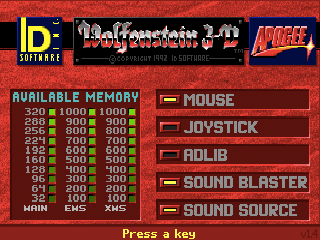
\includegraphics[width=\textwidth]{screenshots/wolf_screen2.png}
  }  
\caption{Dual-monitor: Screen 2.}
\label{fig:dm1}
\end{figure}



 
 
 




\section{Graphics assets}
The graphic assets are divided as follow:
\begin{itemize}
\item 2D Menus items.
\item 3D Action phase items.
\item Wall textures.
\item Entities animations.
\end{itemize}
Those were the work of Adrian Carmack and Kevin Cloud. All of the work was done with Deluxe Paint (from Electronic Arts) on high-end 386 DX computers. 

\begin{figure}[H]
  \centering
 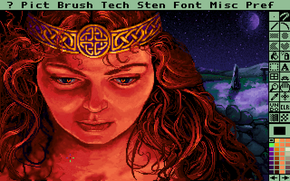
\includegraphics[width=\textwidth]{imgs/deluxe_paint.png}
 \caption{Deluxe Paint tool, used to draw all assets in the game.}
\end{figure}



Since the VGA is palette based (colors a not specific via RBG but by indices pointing to a pallete), the most difficult task was not to draw everything but to make the key decision of what colors would go in the palette\footnote{Some games (such as Monkey island) used many palettes depending on the section of the game but id went for a simple solution: One palette for the whole game.}.\\
\begin{figure}[H]
  \centering
 
\includegraphics[width=\textwidth]{imgs/palette.png}
 \caption{The Game palette: Horizontal from 0x00 to 0x0F, verticall from 0x00 to 0xF0. The blue gradiant starts at 0xF00 and ends at 0xFE. 0xFF (represented in pink) is transparent color and always skipped during rendition.}
\end{figure}

All assets were hand drawn:\\
\begin{fancyquotes}
We didn't have any scanning tools at the time.\\
\\
\textbf{John Carmack - Programmer}
\end{fancyquotes}
\\
I was unable to get in touch with Adrian Carmack or Kevin Cloud but I would have loved to know if they have some sort of stylus or if he was just very good with a mouse.\\

\section{Asset workflow}
Once all the Deluxe Paint images were ready, a tool, IGRAB-ED, packed all the ILBMs files and generated a C header file:\\
 The program could reference an asset directly by using its macro.\\
\begin{figure}[H]
\centering
 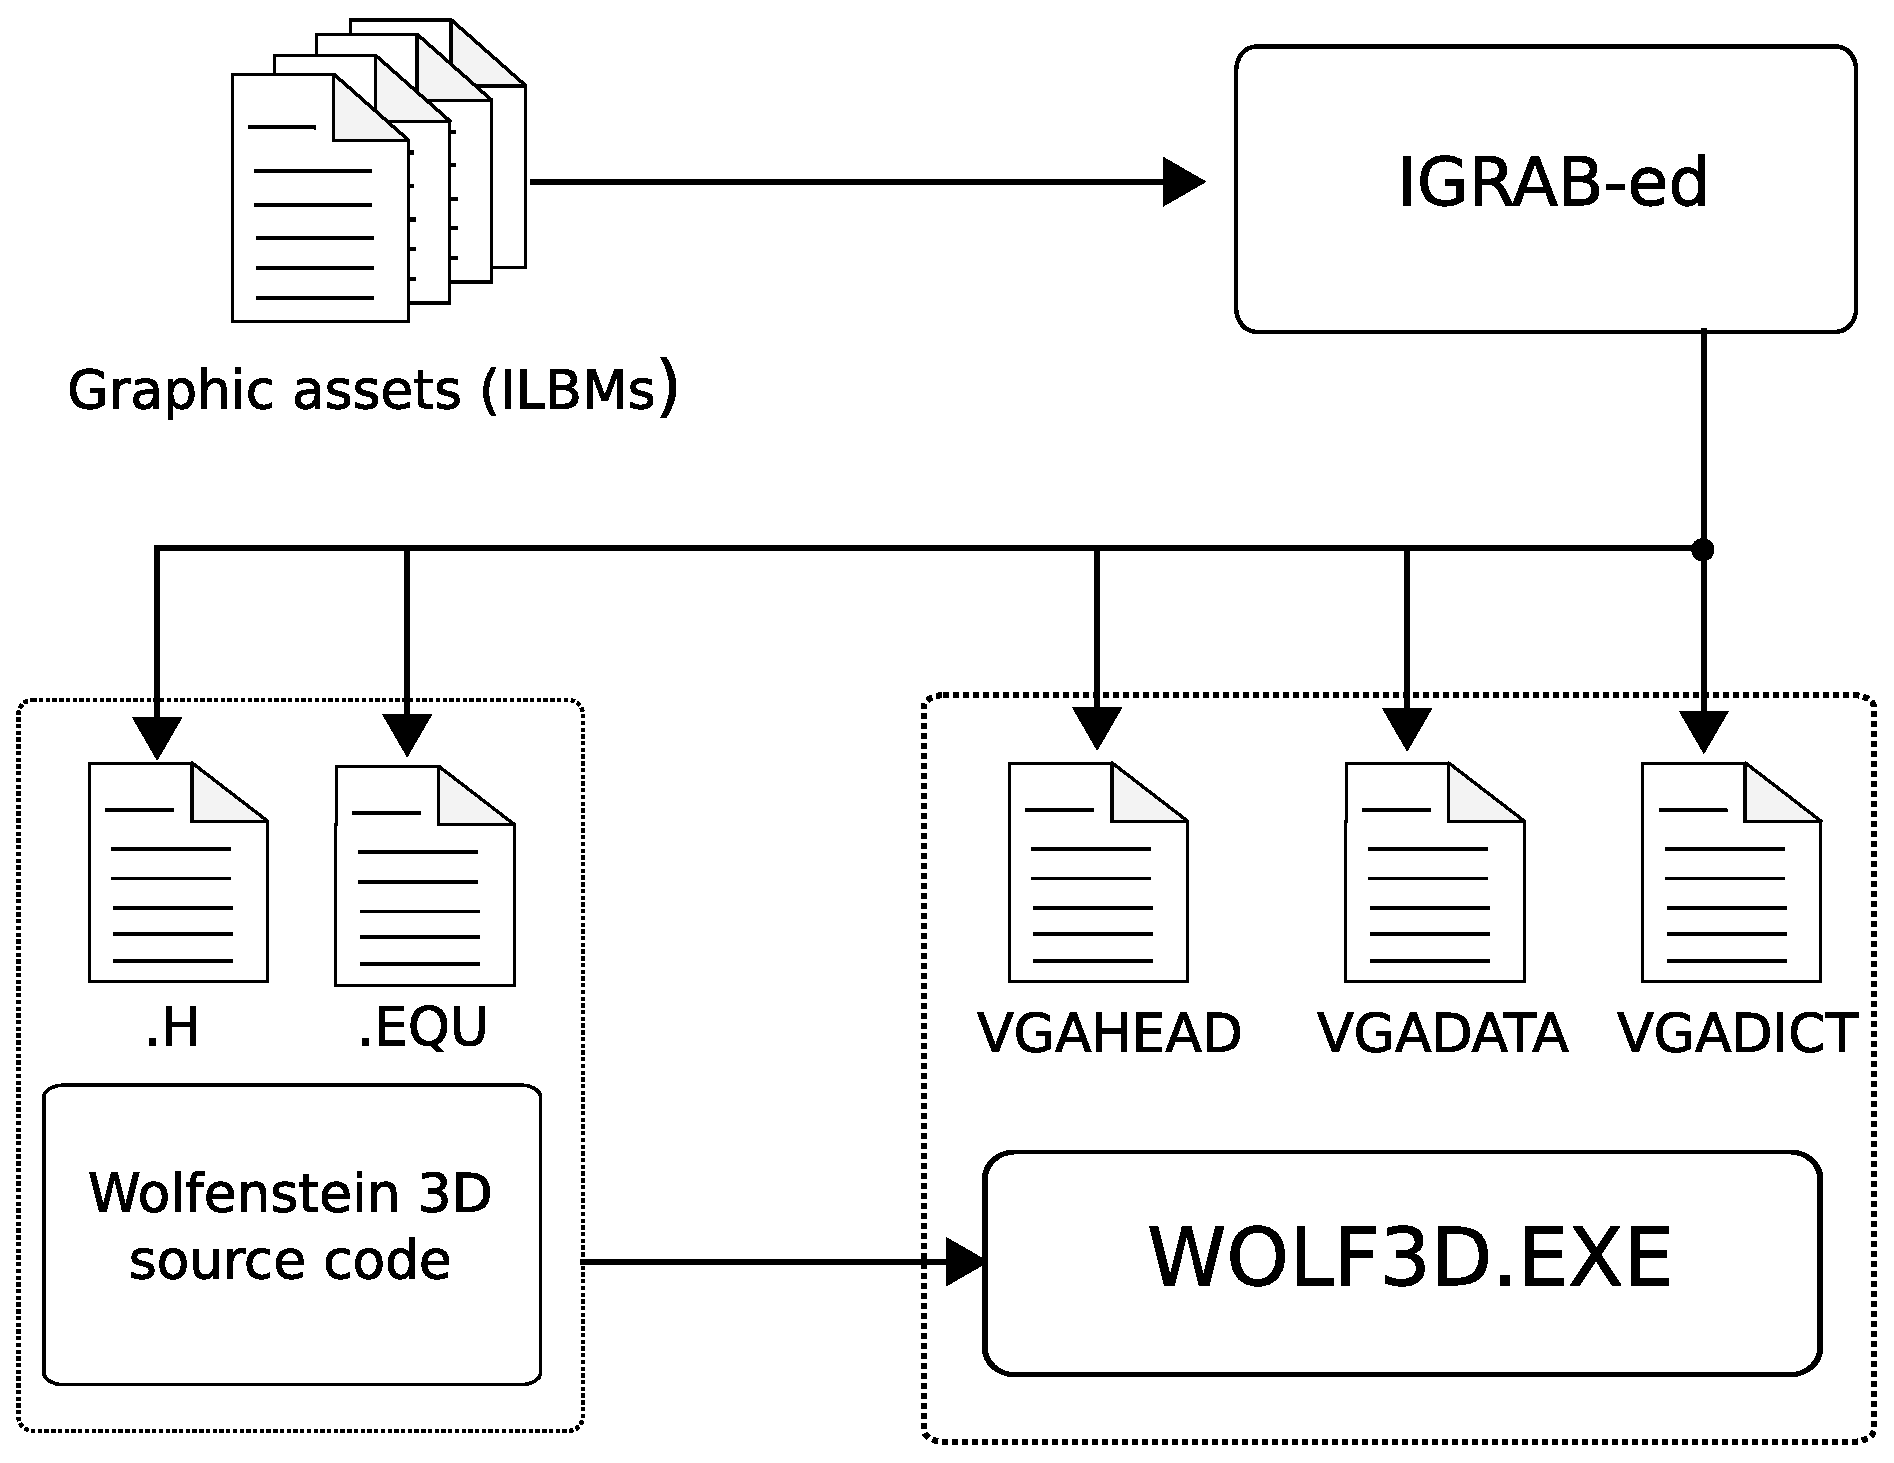
\includegraphics[width=\textwidth]{imgs/drawing_plain.eps}
 \caption{Assets creation} \label{fig:mips}
 \end{figure}

\begin{minipage}{\textwidth}
 \lstinputlisting[language=C]{code/assets_header.c}\par
 \end{minipage}
 
 In the engine, assets usage were "hardcoded" via the enum. This way to work was efficient: Once the name was used in the engine, the assets would be changed and repackaged thanks to the enum indirection layer:\\
 \par
 \begin{minipage}{\textwidth}
 \lstinputlisting[language=C]{code/assets_usage.c}\par
 \end{minipage}

\textbf{\underline{Trivia :}} This system let to issues when the source code was released: The header provided did not match the asset file from the shareware or early version of Wolfenstein 3D: The header released were from Spears of Destiny. You can see the kind of graphic mess this let to in the appendix "Let's compile like it is 1994".\\




\begin{figure}[H]
\centering
      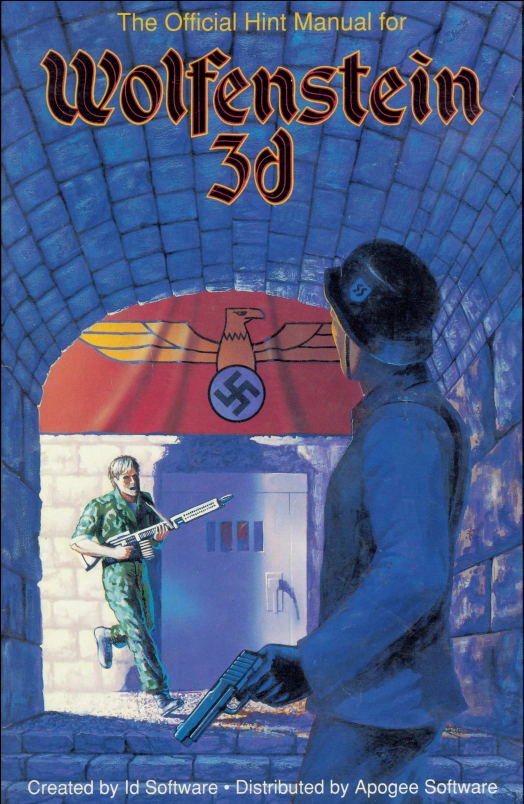
\includegraphics[width=0.3\textwidth]{imgs/hint_manual_cover.png}    
\end{figure}
"The Official Hint Manual for Wolfesnteind 3D"\footnote{The manual was entirely designed on a Next ColorStation. It was the only usage of NeXT for wolfenstein 3D (they purchased it in december 1991).} contains many drawing from Tom Hall. These sketches were given to Adrian Carmack who turned them into pixel art.\\

  \begin{figure}[H]
\centering
 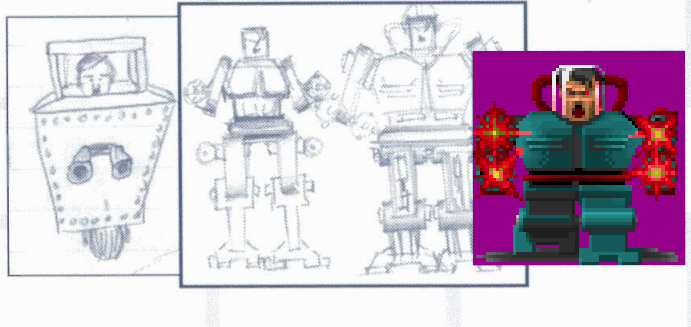
\includegraphics[scale=0.5]{imgs/tom_hall_sketch_adolf.png}
  
\includegraphics[scale=5]{imgs/sprites/adolf.png}
 \end{figure}
 
   \begin{figure}[H]
\centering
 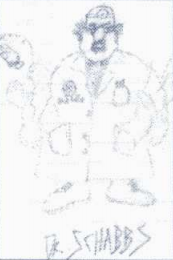
\includegraphics[scale=1]{imgs/tom_hall_sketch_dr_schabbs.png}
   
\includegraphics[scale=10]{imgs/sprites/schabbs.png}
 \end{figure}
 
   \begin{figure}[H]
\centering
 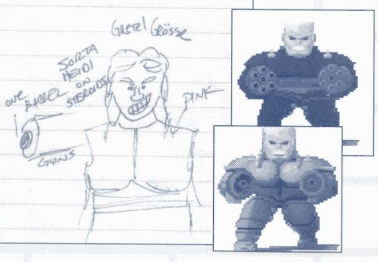
\includegraphics[scale=0.8]{imgs/tom_hall_sketch_gretel.png}\\
 
\includegraphics[scale=2.5]{imgs/sprites/hans_grosse.png}
 
\includegraphics[scale=5]{imgs/sprites/gretel_hanse.png}
 \end{figure}
 
 \begin{fancyquotes}
When Id's Creative Director, Tom Hall gets an idea for a screen, he provides a sketches for Adrian Carmck. Below are some of Tom's early design for the title screen. The third sketch was chosen.\\
\\
\textbf{John Carmack - Programmer}
\end{fancyquotes}

   \begin{figure}[H]
\centering
 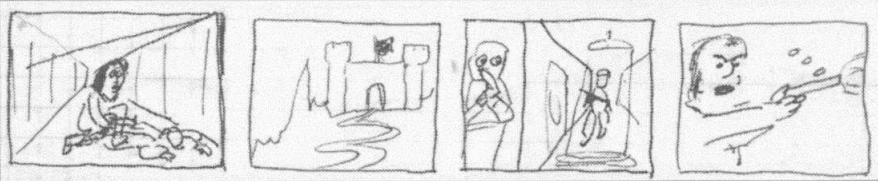
\includegraphics[scale=0.5]{imgs/tom_hall_sketch_intro_screen_genesis.png}
 \par
 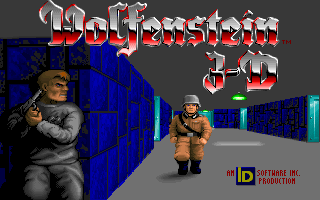
\includegraphics[scale=2]{imgs/sprites/woldf3d.png}
 \end{figure}
 
   \begin{figure}[H]
\centering
 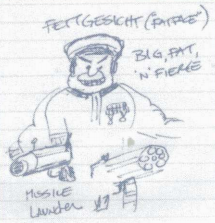
\includegraphics[scale=1]{imgs/tom_hall_sketch_officer.png}

\includegraphics[scale=9]{imgs/sprites/fettgesic.png}
 \end{figure}
 
   \begin{figure}[H]
\centering
 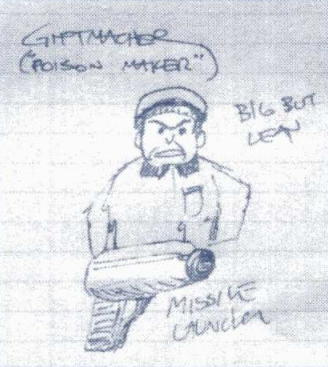
\includegraphics[scale=0.5]{imgs/tom_hall_sketch_officer2.png}
 
\includegraphics[scale=8]{imgs/sprites/giftmacher.png}

 \end{figure}
 
 
The hint book also contains several photos of the team back in the days. Go check it out!













\section{Maps}
Maps were created using the in-house editor called TED5 which is short for Tile EDitor. TED was not create specialy for wolf: It was actually used for Commander Keen serie (yes: a platform scroller).\\

 \begin{figure}[H]
\centering
 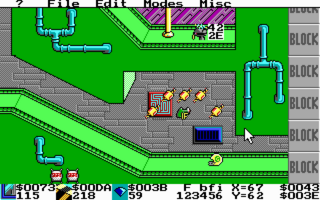
\includegraphics[width=\textwidth]{imgs/ted5_scrolling_map.png}
 \caption{TED used for Commander Keen - side scroller} \label{fig:mips}
 \end{figure}


\begin{figure}[H]
\centering
 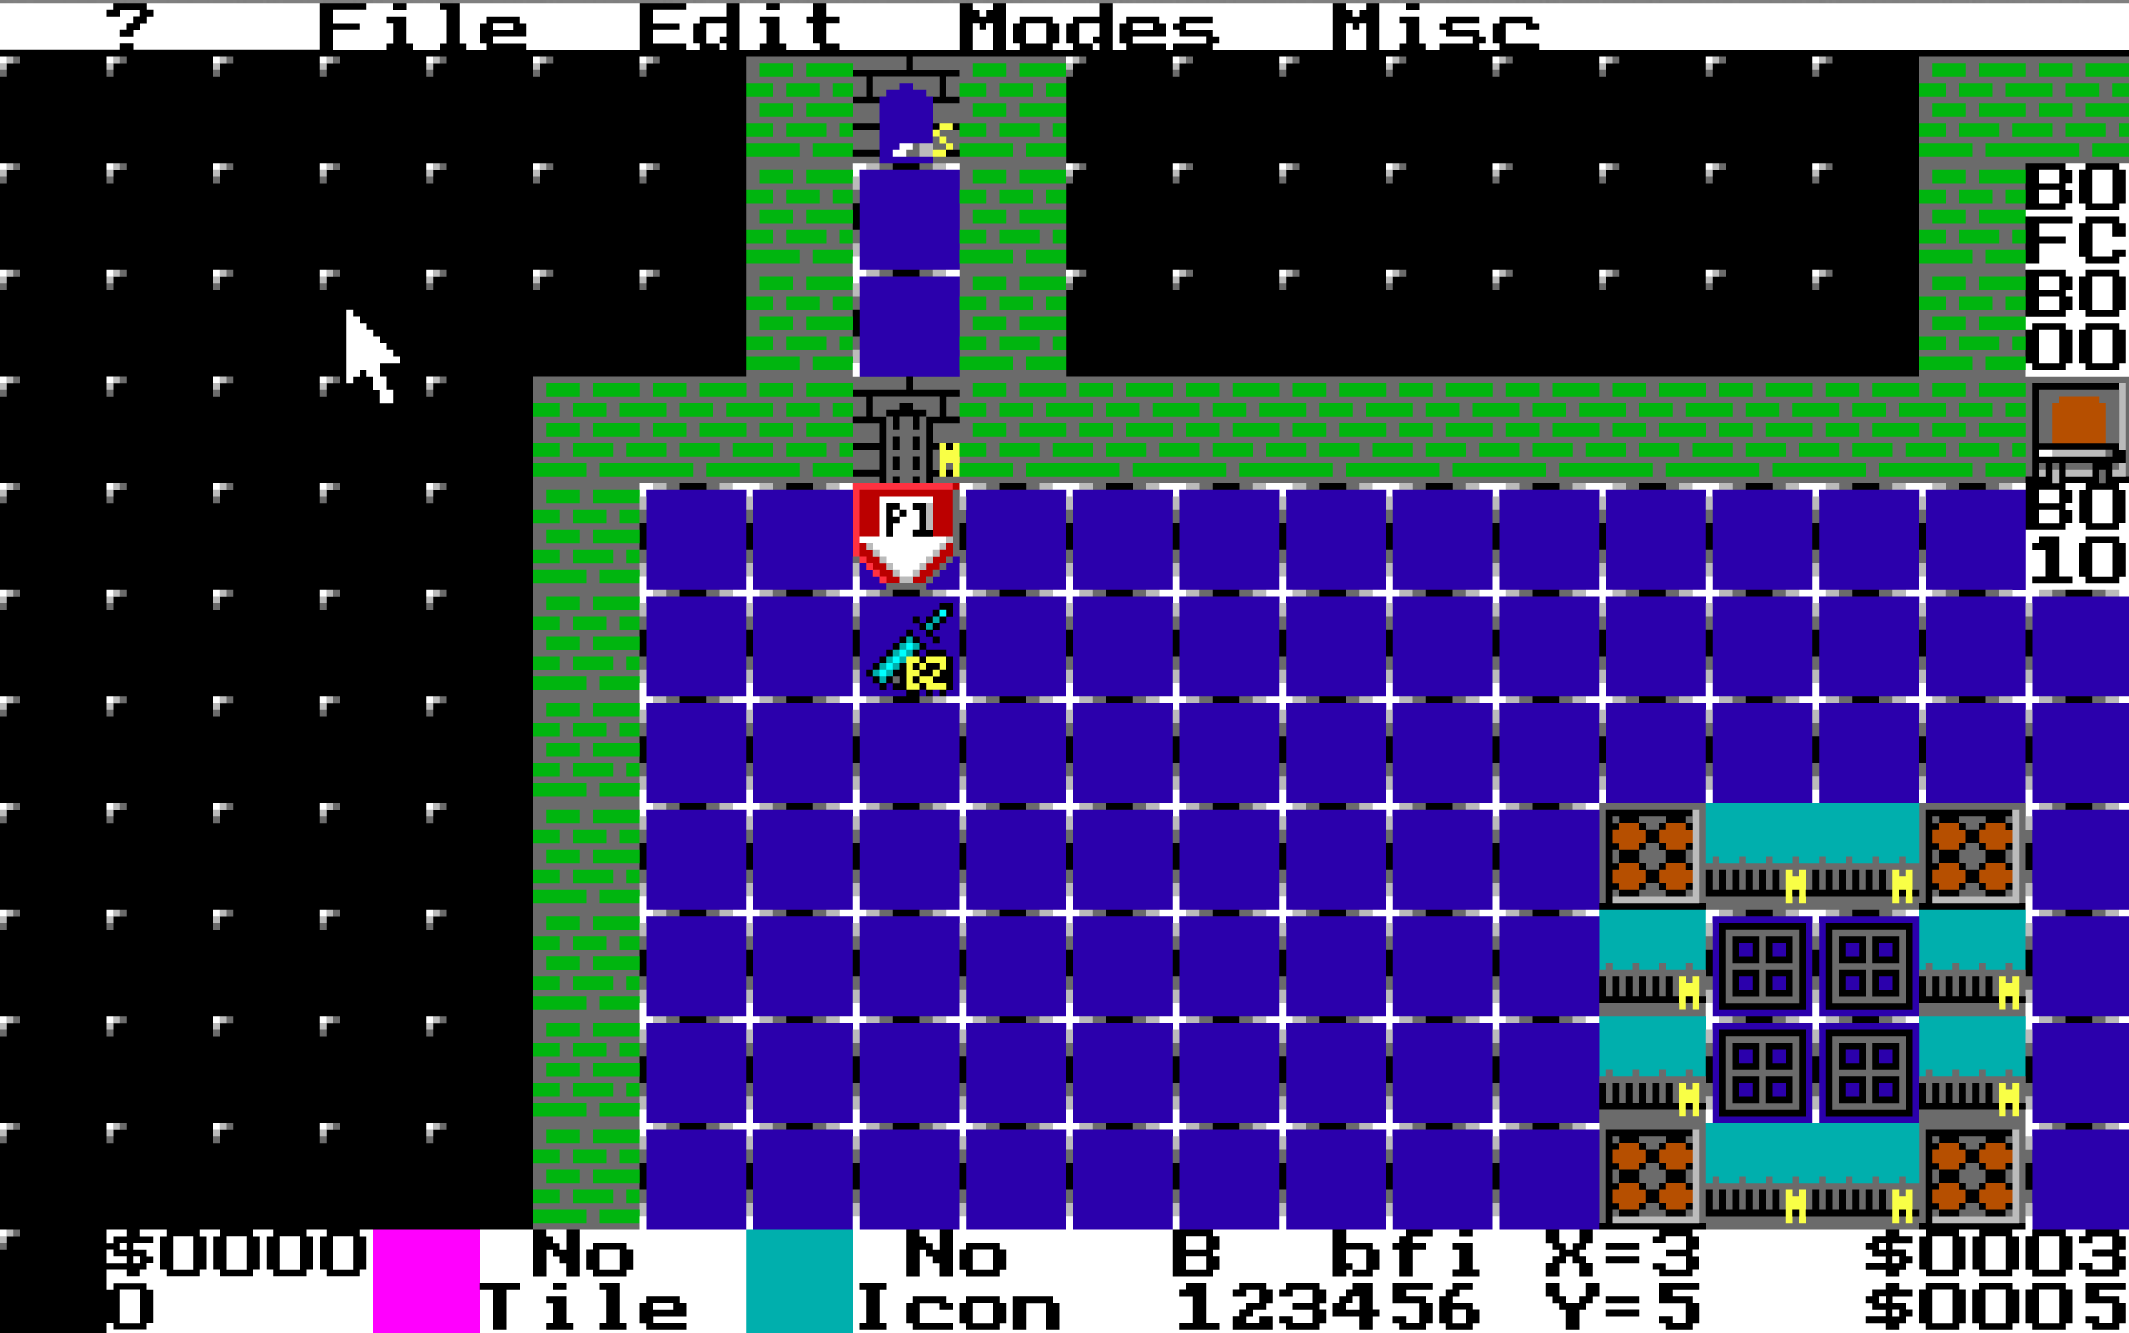
\includegraphics[width=\textwidth]{imgs/TED.png}
 \caption{TED used for top view level design} \label{fig:mips}
 \end{figure}

Since they had been using it for years, the entire team was proficient with TED. It allowed id to make many levels within a small amount of time:

 \begin{fancyquotes}
After talking with Romero and Tom, Scott learned that it was taking the group only about one day to make a level of the game. Ka-chung! Dollar signs! Instead of just three episodes, why not have six? Scott said, “If you can do thirty more levels, it would only take you fifteen days. And we could have it where people could buy the first trilogy for thirty-five dollars or get all six for fifty dollars, or if people buy the first episode and later want the second episodes it will be twenty dollars. So there’s a reason to get them all!” After some consideration, id agreed.
 \textbf{- Masters of Doom}
 \end{fancyquotes}\\

When the engine was licensed to Apogee for Rise of The Triad, TED5 was also used. Tom Halls wrote about it and you can find his comment in the Appendix section.
\par
Everybody worked a little bit on the map but those were mostly the work of John Romero and Tom Hall. John Romero updated the editor TileEDitor (TED). Maps were plans based, 64x64.\\
\par
 \textbf{\underline{Trivia :}} The source code of TED was released several years later. Inspecting the source was a mysterious \codeword{\_TOM.PIC}. Converted to PNG it looks as follow:\\
\begin{figure}[H]
\centering
 
\includegraphics[width=\textwidth]{imgs/_tom.eps}
 \caption{Not so politically correct caricature.} \label{fig:mips}
 \end{figure}
The explanation was provided later by John Romero:\\
 \begin{fancyquotes}
   "Hahahaha! Wow, I forgot all about that picture. I can't believe it's 
in the TED5 source files! It's basically a pic that Adrian drew of Tom 
getting Adrian's dick blasted into his face with Adrian saying "Sorry!". 
It's because Tom and Adrian used to share a worktable together and Tom 
would always bump the table while Adrian was drawing graphics with the 
mouse and Tom would say, "Sorry!" That picture never appears in Ted5 
anywhere.\\
   \\
\textbf{John Romero - Programmer}
 \end{fancyquotes}\\





\section{Business}
I was unable to get in touch with Jay Wilbur. Little is known...for now :) !\\




\section{Sounds}
Despite multiple emails, I was unable to get in touch with Robert Prince. Little is known...for now :) !\\




\section{Office layout}
The team was setup as follow\footnote{Since they played Dungeons \& Dragons a lot, the map is drawn D\&D style.}:
\par
TODO: Insert map of the office as soon as john romero sends it.


\section{Results}
The engine took six weeks to program. TED5 was constantly updated for the six months assets and maps design iterated. The game shipped as follow:
 \begin{figure}[H]
\centering
 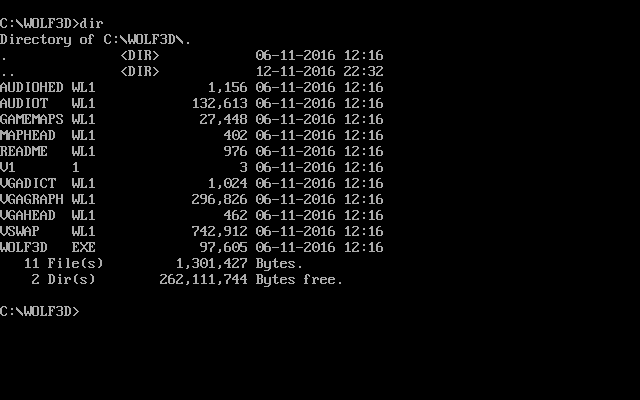
\includegraphics[width=\textwidth]{imgs/result.png}
 \caption{Tile EDitor screen} 
  \end{figure}
  \par
 The files shipped can be divided in five parts:
 \begin{itemize}
 \item WOLF3D.EXE: The Game engine.
 \item VSWAP.WL1: Contains all the assets needed during 3D action phases. The design is clearly inspired by Jason Blochowiak's expereince with Unix systems.
 \item Music files:
     \begin{itemize}
     \item AUDIOHED.WL1 : Offsets to the the individual chunks as signed 32-bit integers.
     \item AUDIOT.WL1: Uncompressed audio chunks. 
     \end{itemize}
\item Maps:
     \begin{itemize}
      \item GAMEMAPS.WL1 
      \item MAPHEAD.WL1: 
      \end{itemize}
\item Pictures:
    \begin{itemize} 
     \item VGADICT.WL1 : Huffman-tree for decopressing the pics.
     \item VGAGRAPH.WL1 : Headers describing where to find the pics.
     \item VGAHEAD.WL1 : Compressed pics lumped together.
     \end{itemize}
\end{itemize}
 \par

\textbf{\underline{Trivia :}} The file extension did have a meeting: 
\begin{itemize}
\item WL1: Shareware
\item WL3: Early three-episode full version
\item WL6: Six-episode full version
\item WJ1: Japanese shareware
\item WJ6: Japanese full version
\item SOD: Spear of Destiny
\end{itemize}
 
\par
 The engine was very tiny and only used 94KB (of it was 64KB dedicated to the Signon screen and 768B for the palette) which means the engine was only 29KB of code.\\
 \par
 All assets combined compressed accounted for 1,207KB.\\
 \par
 Everything was compressed to 645KB to fit on a 3 1/2-inch floppy (these could store 720KB). To make the game fit on one disk was very important given the distribution model
 of the game (shareware) which encouraged people to copy the game and give it to as many people as possible (the game shipped with only one episode, to get the five others
 one had to mail money. The full six episodes fit on two disks. Spears of Destiny would fit on three disks).

\end{document}




